\PassOptionsToPackage{table}{xcolor}
%\documentclass{beamer}
\documentclass[compress]{beamer}
%\usetheme{Epam}
\usetheme{Copenhagen}
\usepackage{xcolor}
\usepackage{listings}
\usepackage{graphicx}
\usepackage[utf8]{inputenc}
\usepackage{datetime}
\usepackage{beamerthemesplit}
%\beamertemplatenavigationsymbolsempty
\usepackage{listingsutf8}
\usepackage{ragged2e}
\usepackage{hyperref}
\lstset{ %
  language=C,                      % the language of the code
%  basicstyle=\ttfamily,           % the size of the fonts that are used for the code
%  basicstyle=\ttfamily\tiny,      % the size of the fonts that are used for the code
  basicstyle=\ttfamily\scriptsize, % the size of the fonts that are used for the code
  numbers=left,                    % where to put the line-numbers
  numberstyle=\tiny\color{gray},   % the style that is used for the line-numbers
  stepnumber=1,                    % the step between two line-numbers. If it's 1, each line 
                                   % will be numbered
  numbersep=5pt,                   % how far the line-numbers are from the code
  %backgroundcolor=\color{gray},   % choose the background color. You must add \usepackage{color}
  showspaces=false,               % show spaces adding particular underscores
  showstringspaces=false,         % underline spaces within strings
  showtabs=false,                 % show tabs within strings adding particular underscores
%  frame=shadowbox,                   % adds a frame around the code
  rulecolor=\color{black},        % if not set, the frame-color may be changed on line-breaks within not-black text (e.g. commens (green here))
  tabsize=4,                      % sets default tabsize to 4 spaces
  captionpos=,                   % sets the caption-position to bottom
  breaklines=false,                % sets automatic line breaking
  breakatwhitespace=false,        % sets if automatic breaks should only happen at whitespace
  title=\lstname,                 % show the filename of files included with \lstinputlisting;
                                  % also try caption instead of title
  keywordstyle=\color{blue},      % keyword style
  commentstyle=\color{mygreen},   % comment style
  stringstyle=\color{magenta},    % string literal style
%  escapeinside={\%*}{*)},        % if you want to add a comment within your code
  inputencoding=utf8,
  extendedchars=\true,
  morekeywords={*,..., restrict, alignof, alignas, bool, true, false, size_t, ssize_t, inline, \_Noreturn, noreturn},
  breakautoindent=false,
  breakindent=1pt,
}

%\setbeameroption{show only notes}
%\usepackage{pgfpages}
%\setbeameroption{show notes}
%\setbeameroption{show notes on second screen=right}

\setbeamertemplate{navigation symbols}{}

\definecolor{oddrow}{RGB}{100,149,237}
\definecolor{evenrow}{RGB}{135,206,250}
\def\mybs{\textbackslash}
\newcommand{\qq}{\symbol{34}} % the decimal ascii code for "
\newcommand{\sq}{\symbol{39}} % the decimal ascii code for '

\makeatletter
\newcommand{\rmnum}[1]{\romannumeral #1}
\newcommand{\Rmnum}[1]{\expandafter\@slowromancap\romannumeral #1@}
\newcommand{\inc}{\symbol{45}\symbol{45}}
\newcommand{\dec}{\symbol{43}\symbol{43}}
\newcommand{\lsh}{\symbol{60}\symbol{60}}
\newcommand{\rsh}{\symbol{62}\symbol{62}}
\makeatother

\newcommand{\specialcell}[2][c]{%
  \begin{tabular}[#1]{@{}c@{}}#2\end{tabular}}
\newcommand{\specialcellhl}[2][l]{%
  \begin{tabular}[#1]{@{}l@{}}#2\end{tabular}}
\newcommand{\specialcellhc}[2][c]{%
  \begin{tabular}[#1]{@{}c@{}}#2\end{tabular}}

\definecolor{mygreen}{rgb}{0,0.6,0}
\definecolor{olive}{rgb}{0.3, 0.4, .1}
\definecolor{fore}{RGB}{249,242,215}
\definecolor{back}{RGB}{51,51,51}
\definecolor{title}{RGB}{255,0,90}
\definecolor{dgreen}{rgb}{0.,0.6,0.}
\definecolor{gold}{rgb}{1.,0.84,0.}
\definecolor{JungleGreen}{cmyk}{0.99,0,0.52,0}
\definecolor{BlueGreen}{cmyk}{0.85,0,0.33,0}
\definecolor{RawSienna}{cmyk}{0,0.72,1,0.45}
\definecolor{Magenta}{cmyk}{0,1,0,0}

\newcommand{\kwblue}[1]{\texttt{\textcolor{blue}{#1}}}
\newcommand{\kwblack}[1]{\texttt{\textcolor{black}{#1}}}
\newcommand{\kwred}[1]{\texttt{\textcolor{red}{#1}}}
\newcommand{\kwmagenta}[1]{\texttt{\textcolor{Magenta}{#1}}}

%\newcommand{\hdr}[1]{\textless{#1}\textgreater{}}
\newcommand{\hdr}[1]{\textless{\kwmagenta{#1}}\textgreater{}}

\author[\href{mailto:vasili_slapik@epam.com}{Vasili Slapik}]{\texorpdfstring{Vasili Slapik\newline\href{mailto:vasili_slapik@epam.com}{vasili\_slapik@epam.com}}{Vasili Slapik}}


\title{\Rmnum{8}. Structures and unions}

\begin{document}

%TODO: struct, unions and enums define namespaces
%TODO: slide for packed structs with the whole at the end ...
%TDOD: designed initializator for structures, GCC version using member:value syntax (not .member = value)


%%%%%%%%%%%%%%%%%%%%%%%%%%%%%%%%%%%%%%%%%%%%%%%%%%%%%%%%%%%%%%%%%%%%%%%%%%%%%%%%%
\frame{\titlepage}
%%%%%%%%%%%%%%%%%%%%%%%%%%%%%%%%%%%%%%%%%%%%%%%%%%%%%%%%%%%%%%%%%%%%%%%%%%%%%%%%%
\begin{frame}{Structure declaration}
    \lstset{
        numbers=none,
    }
    \only<1>{
        \lstinputlisting{08_struct_decl_syntax.txt}
    }
    \only<2>{
        \lstinputlisting{08_struct_decl.c}
    }
    \only<3>{
        \lstinputlisting{08_struct_decl_2.c}
    }
    \lstset{
        numbers=left,
    }
\end{frame}
%%%%%%%%%%%%%%%%%%%%%%%%%%%%%%%%%%%%%%%%%%%%%%%%%%%%%%%%%%%%%%%%%%%%%%%%%%%%%%%%%
\begin{frame}{Operations on structures}
    \only<1>{
        There are several operations defined on structures:
        \begin{itemize}
            \item assign a structure to another structure
            \item pass a structure to a function
            \item return a structure from a function
        \end{itemize}
        \vskip 20pt
        A few more points to mention:
        \begin{itemize}
            \item you can treat an array as a first-class type if put it inside a structure
            \item in general you have to write your own function to compare structures
        \end{itemize}
    }
    %\only<2>{
    %    \lstinputlisting{08_struct_compare.c}
    %}
\end{frame}
%%%%%%%%%%%%%%%%%%%%%%%%%%%%%%%%%%%%%%%%%%%%%%%%%%%%%%%%%%%%%%%%%%%%%%%%%%%%%%%%%
\begin{frame}{Structure members access}
    \lstinputlisting{struct_member_access.c}
\end{frame}
%%%%%%%%%%%%%%%%%%%%%%%%%%%%%%%%%%%%%%%%%%%%%%%%%%%%%%%%%%%%%%%%%%%%%%%%%%%%%%%%%
\begin{frame}{Structure initialization}
    \only<1>{
        %\lstinputlisting[basicstyle=\ttfamily]{08_struct_init.c}
        \lstinputlisting[basicstyle=\ttfamily\tiny]{08_struct_init.c}
    }
    \only<2>{
        \lstinputlisting[basicstyle=\ttfamily\tiny]{08_struct_init_2.c}
    }
\end{frame}
%%%%%%%%%%%%%%%%%%%%%%%%%%%%%%%%%%%%%%%%%%%%%%%%%%%%%%%%%%%%%%%%%%%%%%%%%%%%%%%%%
\begin{frame}{Structure padding}
    \only<1>{
        \lstinputlisting{08_struct_pack.c}
    }
    \only<2>{
        \lstinputlisting{08_struct_padding.c}
    }
    \only<3>{
        \lstset{
            numbers=none,
        }
        \begin{tabular}{llll}
            \specialcellhl{
                \lstinputlisting{08_alignm_png_struct.txt}
            } &
            \specialcellhl{
                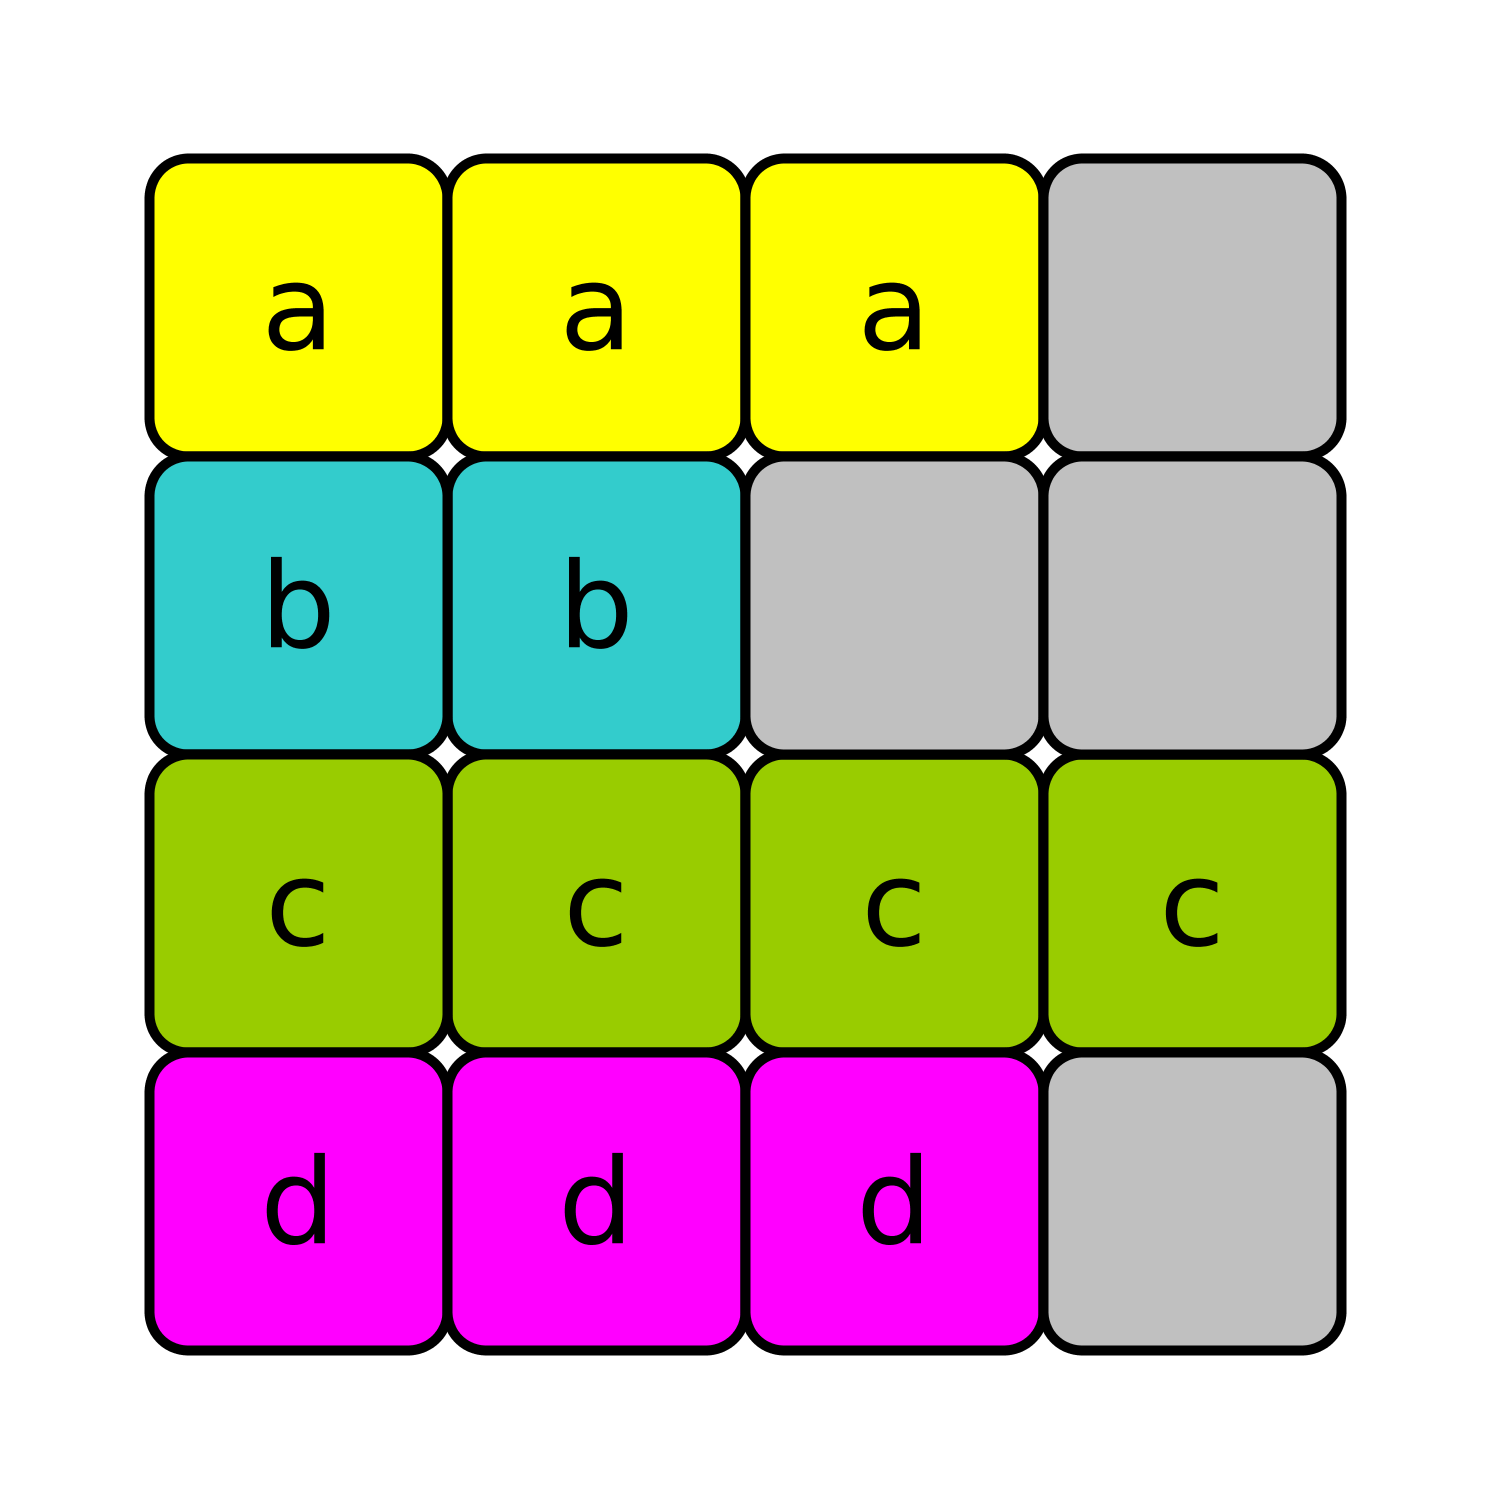
\includegraphics[width=4cm]{08_alignm_02.png}
            } \\
            \specialcellhl{
                \lstinputlisting{08_alignm_png_struct_packed.txt}
            } &
            \specialcellhl{
                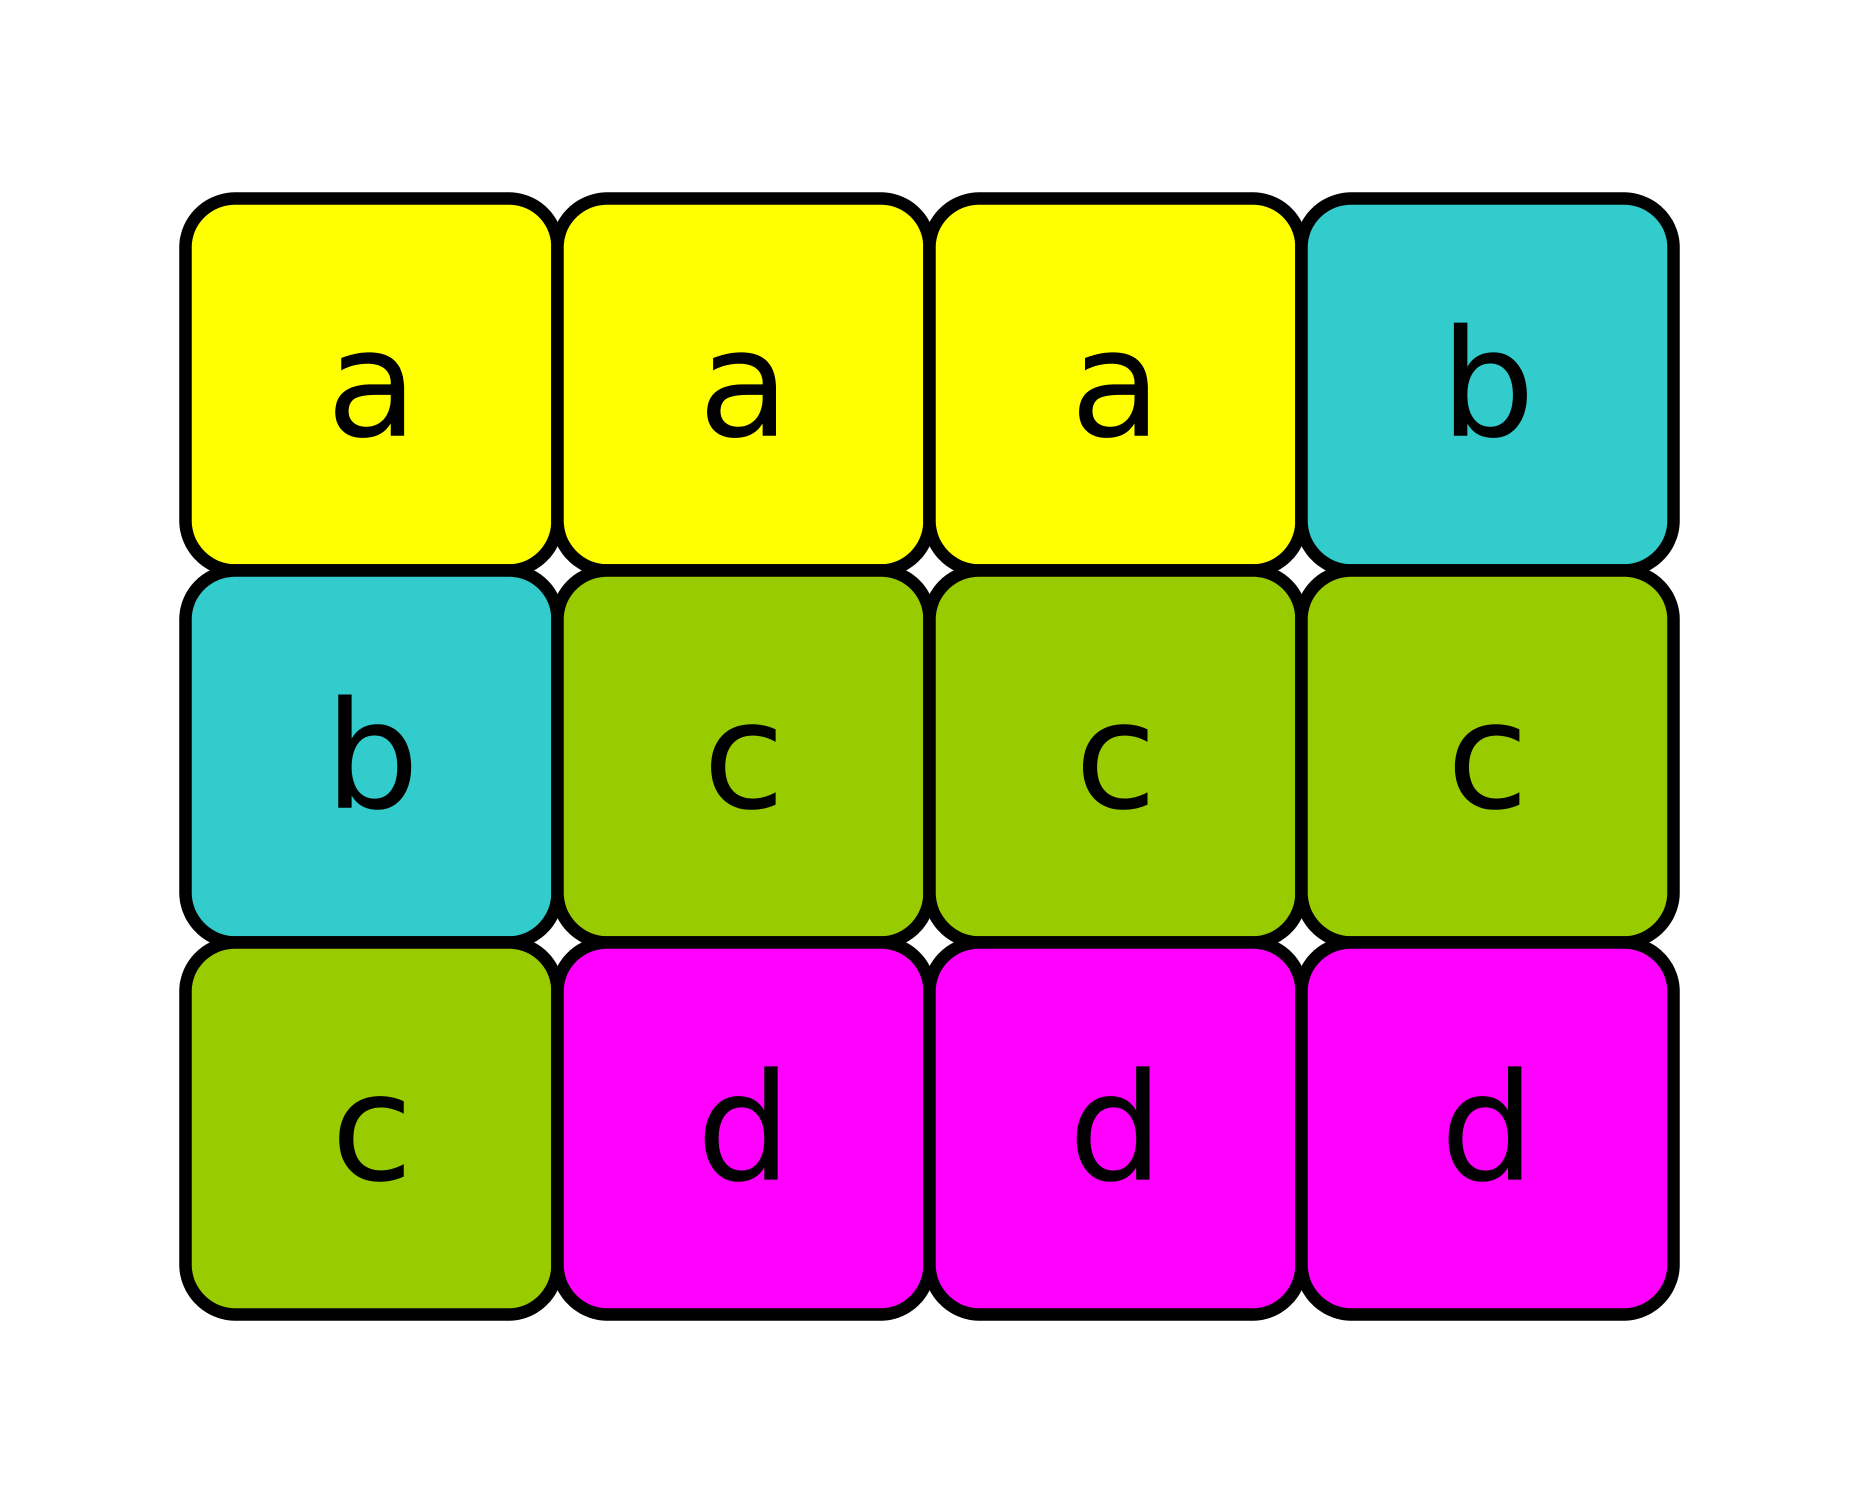
\includegraphics[width=4cm]{08_alignm_01.png}
            } \\
        \end{tabular}
        \lstset{
            numbers=left,
        }
    }
    \only<4>{
        \begin{center}
            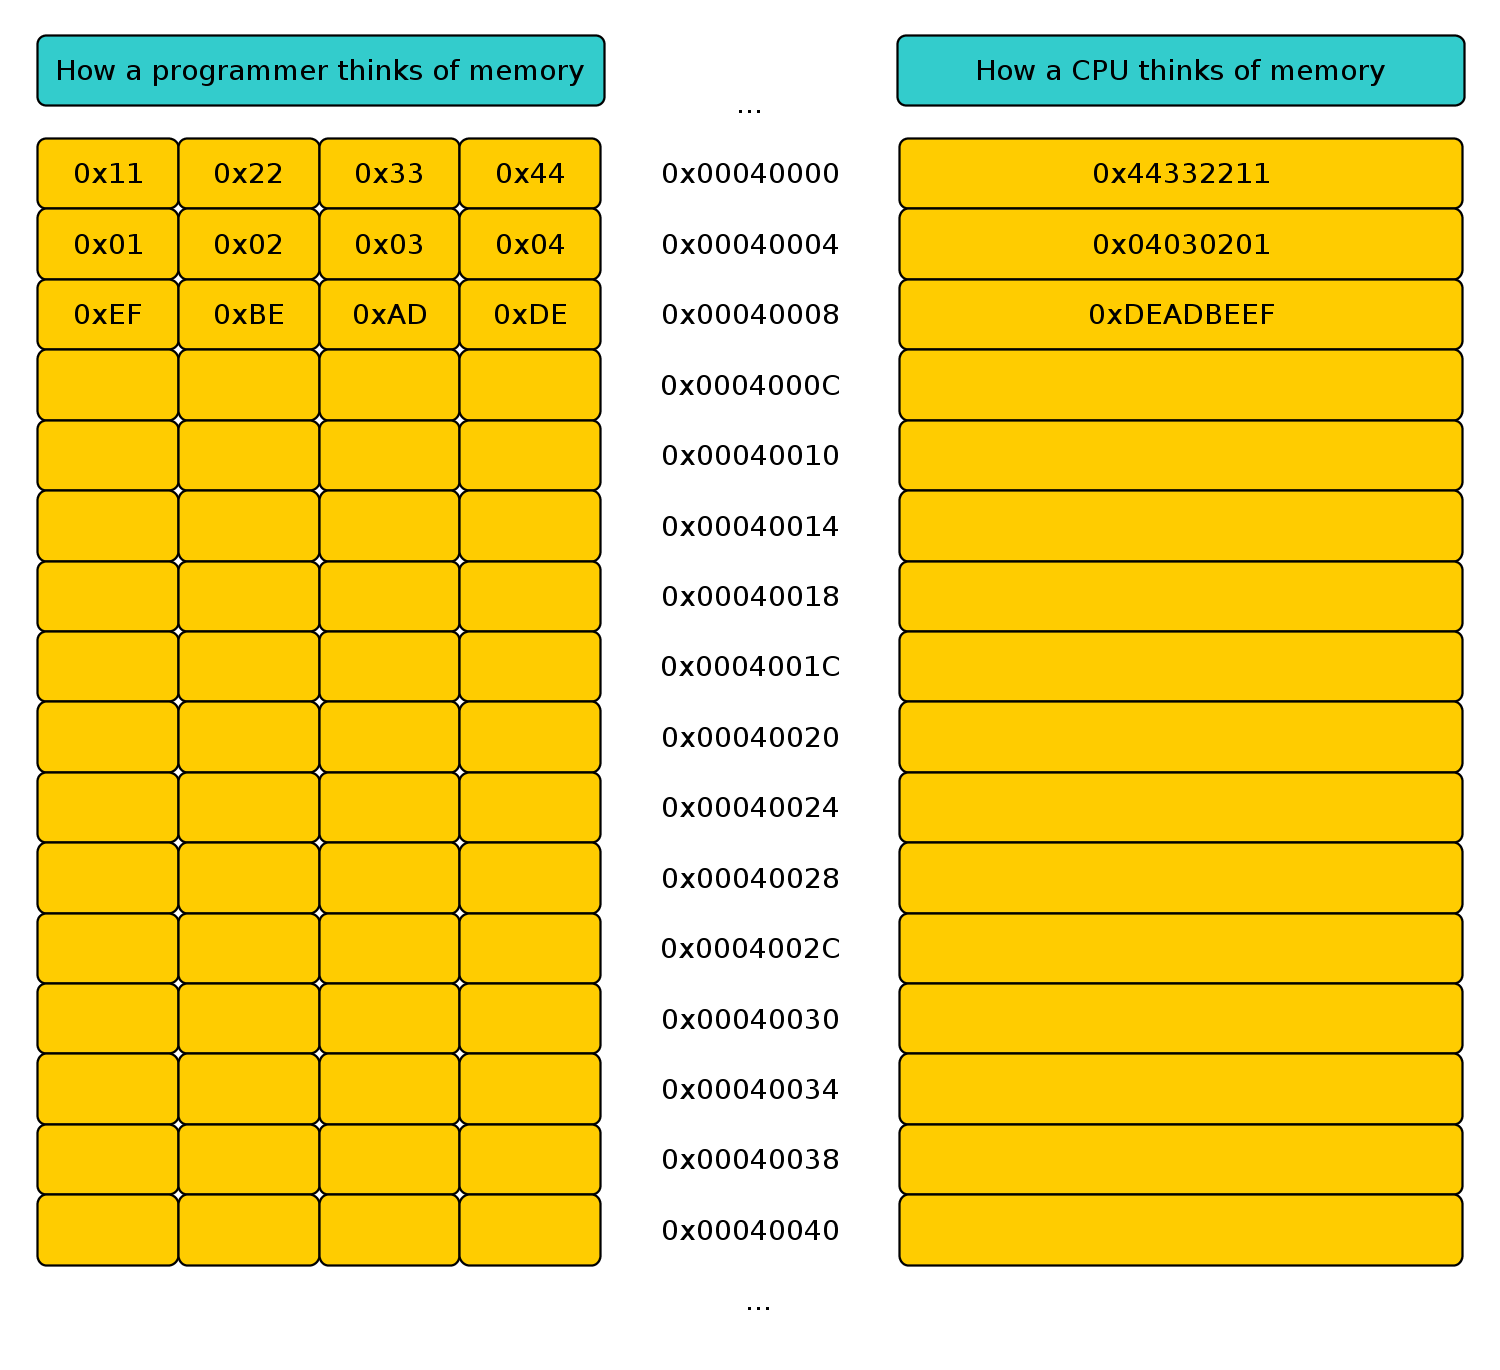
\includegraphics[width=8.5cm]{08_alignm_expl.png}
        \end{center}
    }
    \only<5>{
        Can a compiler rearrange the members inside a structure in order to avoid padding? The answer is "No".
        \begin{block}{C11 \textsection{6.7.2.15}}
            Within a structure object, the non-bit-field members and the units in which bit-fields
            reside have addresses that increase in the order in which they are declared.
        \end{block}
    }
\end{frame}
%%%%%%%%%%%%%%%%%%%%%%%%%%%%%%%%%%%%%%%%%%%%%%%%%%%%%%%%%%%%%%%%%%%%%%%%%%%%%%%%%
\begin{frame}{Bit fields}
    \only<1>{
        \lstinputlisting{08_bit_field_example.c}
    }
    \only<2>{
        \begin{itemize}
            \item the total number of bits in a single bit field must not exceed the total number of bits in its declared type
            \item bit fields do not have addresses (can't use \kwblue{\&} operator on them)
            \item \kwblue{sizeof} operator may not be applied to bit fields
            \item it is not allowed to define an array of bit fields
        \end{itemize}
        \begin{block}{Kernighan \& Ritchie \textsection{6.9}}
            Almost everything about [bit] fields is implementation-dependent.
        \end{block}
        \begin{itemize}
            \item it is implementation defined whether a bit field declared as type \kwblue{int} is signed or unsigned
            \item the packing order of bitfields is implementation defined
            \item whether or not a bitfield may cross a storage unit boundary is implementation defined
        \end{itemize}
    }
    \only<3>{
        \lstinputlisting[basicstyle=\ttfamily\tiny]{08_bits_manipulation_bitfields.c}
    }
    \only<4>{
        \lstinputlisting[basicstyle=\ttfamily\tiny]{08_bits_manipulation_macros.c}
    }
\end{frame}
%%%%%%%%%%%%%%%%%%%%%%%%%%%%%%%%%%%%%%%%%%%%%%%%%%%%%%%%%%%%%%%%%%%%%%%%%%%%%%%%%
\begin{frame}{Unions}
    \only<1>{
        \lstinputlisting[numbers=none]{08_union_decl_syntax.txt}
    }
    \only<2>{
        \lstinputlisting[numbers=none]{08_union_example.c}
    }
    \only<3>{
        \lstinputlisting{08_union_example_2.c}
    }
    \only<4>{
        \lstinputlisting[basicstyle=\ttfamily\tiny]{08_union_example_3.c}
    }
\end{frame}
%%%%%%%%%%%%%%%%%%%%%%%%%%%%%%%%%%%%%%%%%%%%%%%%%%%%%%%%%%%%%%%%%%%%%%%%%%%%%%%%%
\begin{frame}{Tagged unions}
    \only<1>{
In computer science, a \kwblue{tagged union}, also called a variant, variant record, choice type, discriminated union, disjoint union, sum type or coproduct, is a data structure used to hold a value that could take on several different, but fixed, types. Only one of the types can be in use at any one time, and a tag field explicitly indicates which one is in use.
    }
    \only<2>{
        \lstinputlisting{08_tagged_union.c}
    }
\end{frame}
%%%%%%%%%%%%%%%%%%%%%%%%%%%%%%%%%%%%%%%%%%%%%%%%%%%%%%%%%%%%%%%%%%%%%%%%%%%%%%%%%
\begin{frame}{Type punning}
    \only<1>{
        \lstinputlisting[numbers=none]{08_union_example.c}
    }
    \only<2>{
In computer science, \kwblue{type punning} is a common term for any programming technique that subverts or circumvents the type system of a programming language in order to achieve an effect that would be difficult or impossible to achieve within the bounds of the formal language.
    }
    \only<3>{
        \begin{block}{C11 \textsection{6.5.2.3}}
If the member used to read the contents of a union object is not the same as the member last used to
store a value in the object, the appropriate part of the object representation of the value is reinterpreted
as an object representation in the new type as described in 6.2.6 (a process sometimes called "type
punning")
        \end{block}
    }
\end{frame}

\end{document}
